\documentclass[conference]{IEEEtran}
\usepackage{amsmath,amssymb,booktabs,graphicx,xcolor}
\usepackage[hidelinks]{hyperref}
\usepackage{url}
\usepackage{balance}
\usepackage{iftex}
\ifXeTeX
\usepackage{fontspec}
\setmainfont{texgyretermes-regular.otf}[BoldFont=texgyretermes-bold.otf,ItalicFont=texgyretermes-italic.otf,BoldItalicFont=texgyretermes-bolditalic.otf]
\setsansfont{texgyreheros-regular.otf}[BoldFont=texgyreheros-bold.otf,ItalicFont=texgyreheros-italic.otf]
\setmonofont{texgyrecursor-regular.otf}[BoldFont=texgyrecursor-bold.otf]
\fi
\definecolor{forest}{RGB}{32,75,64}
\title{Maintaining Source-Linked Evidence Views for Agent Memory}
\author{}
\begin{document}
\maketitle
\begin{abstract}
An agent may need several observations from an execution history to support its next decision. Each observation costs context tokens and may become unavailable independently. We demonstrate a SQLite system that selects a bounded evidence view, exposes its source dependencies and determines whether an exclusion requires rebuilding the view. The selector protects a ranked prefix and packs its remaining budget using learned utilities. We derive a necessary and sufficient reuse condition for deletions when costs, ordering and utilities are fixed. A cheaper sufficient test indexes the chosen units and the first unit that blocked prefix growth. On 2,528 single-source exclusions across 40 traces, this test reused 2,041 packets, matched every full recomputation and reduced aggregate serving time by a factor of 5.16. Visitors can exclude a source, compare plans, trace a replacement to its origin and audit the resulting evidence coverage independently.
\end{abstract}

\section{Why maintain the evidence packet?}

An execution trace may record a tool invocation in one event and its outcome in another. A later question can depend on parts of both. A memory system must decide which units to admit into the context of a reader, subject to the actual cost of each unit. After an observation becomes unavailable, a system that exposes its dependencies should also explain whether the reader can still receive the same context. Losing an unselected candidate can matter if its absence changes the selection rule.

In one 2,048-token packet, excluding a tool call replaces unit 11 with unit 19. Token cost and annotated coverage stay constant. In another scenario, an excluded source carries no dependency of the materialized result, so no optimizer call is needed. The visitor can inspect both outcomes on individual traces.

Prior work supplies three parts of this problem. Wang et al.\ use source-aligned provenance units and a residual relational graph model to recover supporting spans in execution traces \cite{wang}. Bala distinguishes retrieval from the evidence that actually survives packing for a reader \cite{bala}. Feng et al.\ study sets of evidence that supply missing information in a captured coding-agent state \cite{feng}. Our system operates at a different point in the data path. Once the source-linked candidates have costs, ranks and utilities, it materializes the evidence packet and monitors which source exclusions can affect its contents.

The database question resembles maintenance of materialized top-$k$ views. Yi et al.\ maintain additional ranked tuples to reduce costly refills after updates \cite{topk}. Here a selected packet depends on a cumulative-cost prefix and on a second, constrained optimization. A single rank cutoff does not capture these dependencies. TAPE demonstrates temporal graph memory for personal agents \cite{tape}. Our interface exposes the provenance and token cost of an execution-memory view, with a separate control for checking its consistency after an exclusion.

\begin{figure}[t]
\centering
\setlength{\fboxsep}{4pt}
\begin{tabular}{@{}c@{}}
\fcolorbox{forest}{white}{\parbox{.88\columnwidth}{\centering \textbf{Public execution trace}\\Events, argument/output fields and character offsets}}\\[-1pt]
$\downarrow$\\[-2pt]
\fcolorbox{forest}{white}{\parbox{.88\columnwidth}{\centering \textbf{Read-only SQLite projection}\\Unit, source span, directed relation, cost, rank, utility}}\\[-1pt]
$\downarrow$\\[-2pt]
\fcolorbox{forest}{white}{\parbox{.88\columnwidth}{\centering \textbf{Materialized view and source dependencies}\\Protected prefix, packed suffix and prefix boundary}}\\[-1pt]
$\downarrow$\\[-2pt]
\fcolorbox{forest}{white}{\parbox{.88\columnwidth}{\centering \textbf{Live visitor controls}\\Exclude a source, inspect a unit, compare maintenance plans}}\\
\end{tabular}
\caption{Serving architecture. A separate evaluator receives the resulting unit IDs and compares their source intervals with a private annotation table on demand. The selection path has no access to that table or to the bodies of tool calls.}
\label{fig:system}
\end{figure}

\section{Selection and source dependencies}

\subsection{Materializing a view}
For a query $q$, the input is an ordered set of candidates. Unit $i$ has token cost $c_i\geq 0$, learned utility $u_i$ and one or more source intervals. An interval identifies an event, a JSON field and a half-open range of character offsets. Several units can refer to the same source. Their selected token costs add even if their source intervals overlap. Evaluation later merges overlapping intervals in source coordinates to avoid double counting support.

Let $B$ be the token budget and $T\leq B$ the prefix threshold. In rank order, the reader protects the longest consecutive prefix $H$ whose total cost stays within $T$. If a next unit exists, the first unit that fails to enter $H$ is its \emph{boundary}. Full-budget first-fit is a strong baseline. It scans the same ordered candidates and admits each one whose cost fits the remaining budget. Our alternative reserves some freedom to exchange expensive early units for combinations of later ones.

The reader uses graph-informed rank and type, unit cost, dense rank, the graph-informed score and its gap from the leading item, and pool size. A gradient-boosted tree model fits evidence membership on 3,894 training queries with equal total weight per query. At serving time a monotone softplus transform converts the fitted log-odds to additive utility. Model fitting and graph projection occur before the visitor opens a trace. Candidate utility measures a training objective and cannot by itself establish joint sufficiency.

Write $C=B-\sum_{i\in H} c_i$. On the remaining candidates the selector maximizes $\sum_i u_i x_i$ subject to $\sum_i c_i x_i\leq C$ and $x_i\in\{0,1\}$. A standard exact dynamic program updates the value at each integer capacity. An explicit tie rule keeps the existing solution when a later candidate gives the same value. Selected IDs are returned in their original rank order. Threshold selection on 580 validation queries gave $T=1,024$ at $B=2,048$. Other thresholds trade a larger fixed prefix against additional freedom for the optimizer. The contribution here is a materialized packet with auditable source dependencies and maintenance rules.

\subsection{When can an exclusion change a packet?}
Let $P$ denote the stored packet and $D$ the set of candidate IDs removed by one or more source exclusions. Surviving candidates retain their order, costs and utilities. The budget, threshold and deterministic preference among tied solutions also stay fixed. Let $H'$ be the protected prefix recomputed on the remaining candidates.

\textbf{Reuse criterion.} The ordered packet is unchanged exactly when
\[
           D\cap P=\varnothing \quad\text{and}\quad H'\subseteq P.
\]
If a selected unit is removed, its ID cannot survive. If the new prefix contains a previously unselected unit, the new packet must contain that unit. For sufficiency, the first condition implies that all members of $H$ survive. Deletions can extend this prefix, so $H\subseteq H'$. By the second condition the old optimum contains every newly mandatory unit and remains feasible. Every packet feasible under the new requirement was already feasible before deletion. On these nested feasible families a previous optimum remains optimal, and the stable tie rule preserves its identity. Rank order of the surviving units is unchanged, giving equality of the ordered packets. The proof assumes exact comparisons and a stable tie order. A signed 64-bit implementation with fixed-point Q32 utilities reproduced all 10,000 original packets and all 108,204 deletion outcomes. The maximum tested utility sum was 13,789,213,370. Arbitrary floating-point summation orders do not inherit this guarantee.

There is a cheaper sufficient certificate. Index every source of a selected unit and every source of the boundary unit. When an exclusion touches neither, the prefix and its boundary survive and the suffix loses only unselected items. The old packet can be returned following a dependency lookup. A hit triggers full recomputation. The certificate is conservative. Excluding the boundary can admit a previously optional unit that the packet already contained. In that case the exact criterion can still certify reuse.

A four-unit example illustrates the boundary. Let the budget be 8, the prefix threshold 4, costs $(3,3,1,5)$ and utilities $(1,1,3,10)$. The original prefix contains only unit 0 and the suffix chooses unit 3. Deleting unselected unit 1 forces the new prefix $(0,2)$. Only 4 tokens remain and unit 3 no longer fits. Monitoring only the chosen IDs would incorrectly return $(0,3)$.

\section{Implementation and visitor interaction}

The application serves a read-only SQLite projection and a Python HTTP interface on the visitor's machine. The \texttt{node} table stores a query-local ID, the hashed graph node ID, role, token cost, rank and precomputed utility. The \texttt{span} and \texttt{origin} tables map units to source hashes, event positions and text intervals. The \texttt{edge} relation stores typed directed links between graph nodes. This schema supports inspecting provenance independently of whether a unit made it into a packet. The selector reads the ordered metadata through a parameterized query. An anti-join removes every candidate incident on an excluded source. The reader can still display the reason that an admitted unit entered the packet and the source range to which it refers.

At startup the projection contains 5,009 units, 2,528 distinct query-source pairs and 10,789 typed execution edges across 40 queries from distinct traces. We chose the first query per trajectory in a fixed hash order, independently of its measured success. ISETrace contains execution-grounded synthetic OS-agent trajectories with generated intents and interactions. Its tool calls were actually executed \cite{ise,wang}. We verified event and field identities and character boundaries against these canonical records. Source exclusions in the demo are hypothetical interventions on the recorded data. Only hashes, offsets, roles and numeric metadata enter the serving database. The visitor can inspect the evidence structure without retrieving raw tool output. The goal of the screen is to show how selection and source exclusion interact on recorded traces.

\begin{figure*}[t]
\centering
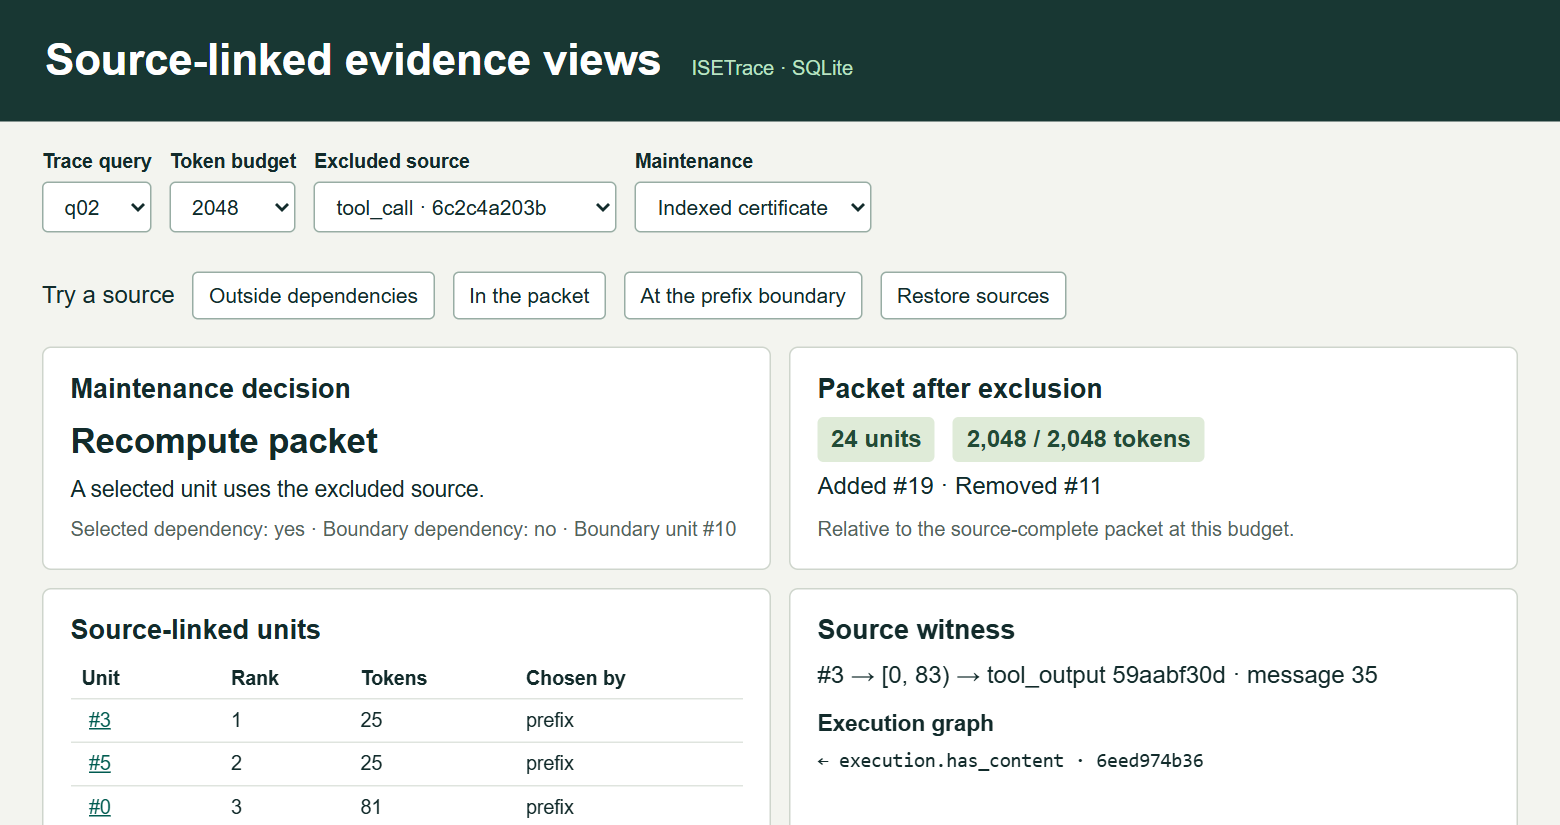
\includegraphics[width=.90\textwidth]{visitor.png}
\caption{Actual visitor console following the exclusion of a source in query q02. The selected dependency forces recomputation. Unit 19 enters and unit 11 leaves at the same 2,048-token cost. The lower panels expose unit ranks and links to original event ranges.}
\label{fig:ui}
\end{figure*}

\subsection{Three visitor scenarios}
\textit{Trace a selected unit.} A visitor opens a query at the validated budget and selects an entry from the packet. The system shows its rank, token cost, how the selector admitted it and the half-open range in its source event. The adjacent panel exposes the directed relationships incident on the original graph node. Visitors can contrast the origin of a protected early unit with one admitted by the optimizer. Changing the budget reruns selection. Because the suffix is reoptimized, additional budget can displace an earlier choice.

\textit{Exclude a source and inspect the plan.} The visitor can choose any available source or start with a source outside the dependency index. In certificate mode the interface reports reuse of the source-complete view. A selected-source example in q02 instead forces recomputation and displays a two-unit exchange (Fig.~\ref{fig:ui}). Switching to the unconditional plan on the same inputs exposes equivalent output under a different execution policy. A third control loads a real boundary-only case in q07. The sufficient certificate conservatively recomputes even though the final packet survives. Returning the source restores the original snapshot. Each exclusion in this console starts from that snapshot.

\textit{Ask what changed for the reader.} A separate audit control runs a fresh selection and compares ordered IDs with the result displayed by the chosen maintenance plan. Only after selection does an evaluator read a separate database of gold intervals. It merges intervals within each event and field and reports covered characters and full support. On q02, selecting a different packet still covers all 60 gold characters. In a second query a visitor can reduce the budget and inspect which source range drops out. This stage poses a different question from whether the database correctly maintained its view.

\section{Measurements and interpretation}
\subsection{Budgeted evidence recovery}
On 2,000 held-out ISETrace memory queries from 1,207 trajectories, all readers use the same candidate units and official source-span metric. Full Support is one when the union of selected source intervals contains every annotated gold interval. We average over five matched dense-retrieval seeds. The first-fit comparator uses the same graph-informed ranker and token costs. It receives the entire budget to admit later items that fit. This control isolates the effect of choosing the packet under a different objective.

\begin{table}[t]
\caption{Evidence recovery under a 2,048-token cap. Values are means across five matched seeds on the complete test.}
\centering\small
\begin{tabular}{lrr}\toprule
Selector & Support (\%) & Tokens/query\\\midrule
Full R-GCN, strict prefix & 78.60 & 1,854.95\\
No adjacency, strict prefix & 79.21 & 1,850.31\\
Full R-GCN, first-fit & 80.44 & 2,039.97\\
No adjacency, first-fit & 81.19 & 2,039.83\\\midrule
Dense order + exact packing & 75.25 & 2,038.61\\
Graph rank-weighted packing & 80.37 & 2,036.40\\
Graph utility/cost greedy & 82.31 & 2,034.63\\
Same-ranker first-fit & 82.19 & 2,039.30\\
Prefix + exact packing & 82.60 & 2,039.12\\
No adjacency + learned packing & 83.07 & 2,039.12\\
\bottomrule\end{tabular}
\label{tab:retrieval}
\end{table}

The graph-informed candidate order and the learned utility each contribute to the observed ordering in Table~\ref{tab:retrieval}. The dense control used its own validation-selected prefix threshold and a separately trained utility model without the graph-derived inputs. The graph rank-weighted control used the same exact optimizer with a descending utility based only on rank. The greedy control ordered remaining units by learned utility per token. These controls couple features and order. Isolating one edge would require a separate intervention.

Against first-fit, the paired difference is $+0.41$ percentage points. The 95\% interval from crossed trajectory and seed resampling is $[-0.23,+1.08]$ points. The interval includes both a small loss and a gain against first-fit. These outcomes quantify the evidence available to a downstream reader. Executable coding-task performance requires a separate experiment. The known test collection was also used in earlier experiments, so transfer to an independently reserved corpus remains an open question.

We evaluated the published full relational graph convolutional network (R-GCN) and the separately trained variant without chunk-adjacency edges on identical queries, budgets and seeds. With the native strict-prefix rule, our packet exceeded them by 4.00 and 3.39 points. Allowing both baselines to use first-fit reduced those gaps to 2.16 points (95\% interval $[0.90,3.45]$) and 1.41 points ($[0.15,2.74]$). Transferring our learned suffix utility to the no-adjacency model's own prefix yielded 83.07\%, the highest point estimate in Table~\ref{tab:retrieval}. This exploratory hybrid suggests that prefix order and packing policy can be investigated separately.

For the same-ranker comparison we additionally measured normalized area under the Full Support curve on the benchmark's logarithmic budget scale, at 256 through 8,192 tokens in powers of two. The budget-dependent selector reached 70.992 against 70.565 with first-fit. The paired difference was $+0.427$ points ($95\%$ interval $[0.102,0.758]$). Each budget produces its own packet. The single-budget result and the integrated result answer distinct questions.

\subsection{View maintenance on a live projection}
First, we compared the portable demo reader with the frozen model on all 40 queries in its operating panel. At 2,048 tokens it reproduced every selected ID in order. Independent interval arithmetic matched the official evaluation for all 40 packets. Their mean size was 2,043.15 tokens and 36 carried complete evidence. An exploratory reduction to 1,024 tokens gave 35 complete packets. Increasing the budget to 3,072 gave 37. The operating point was selected only for the primary budget. A different panel or different query weights can change these fractions.

We then removed each of the 2,528 available query-source pairs independently, always from its source-complete snapshot. The indexed sufficient certificate served the old packet on 2,041 exclusions and recomputed the remaining 487. Ordered IDs matched fresh recomputation on every operation. Three conservative recalculations left the packet unchanged. The cache-hit rate was 80.74\% across exclusions and 77.80\% when each trace was weighted equally.

Both timed plans used the same SQLite data, native exact-packing implementation and precomputed features. Three interleaved repetitions gave 7,584 timed executions per plan. Aggregate full-recomputation time divided by certificate time was $5.16\times$, with a 95\% trajectory-bootstrap interval of $[4.36,6.17]$. Median latency fell from 280.25 to 9.30 microseconds and p95 from 540.29 to 352.82 microseconds. The dependency index added a mean 116 microseconds of setup per query. These are warm, single-host serving measurements. They exclude model training, feature extraction, browser rendering and evidence evaluation. The interactive portable implementation uses a Python optimizer to make the same decisions without native dependencies.

\balance
\begin{table}[t]
\caption{Exact reuse under independent hypothetical source exclusions. The final column counts additional reuse approvals beyond the fast boundary certificate.}
\centering\small
\begin{tabular}{rrrr}\toprule
Sources removed & Cases & Unchanged & Additional\\\midrule
1 & 2,528 & 2,044 & 3\\
2 & 97,676 & 68,336 & 232\\
3 & 4,000 & 1,991 & 12\\
8 & 4,000 & 890 & 17\\
\bottomrule\end{tabular}
\label{tab:exclusions}
\end{table}

The necessary-and-sufficient criterion (Table~\ref{tab:exclusions}) was also tested on 97,676 pairs of source deletions and 4,000 each of triples and eight-source sets. Together with the single exclusions this gave 108,204 comparisons. The criterion identified all 73,261 unchanged packets with zero false positives or negatives. It certified 264 additional unchanged packets compared with the conservative boundary test. Separately, exhaustive enumeration of 20,204 deletion sets on 320 small synthetic pools checked the predicted equivalence, including tied utilities. On the real panel an index monitoring only selected units happened to produce the correct outputs, although the counterexample above establishes its limits. The measured speedup belongs to the conservative single-source plan. Dynamic changes to rank, utility, cost or budget require a fresh snapshot or a separate maintenance argument.

\section{Scope of the demonstration}
Repeated reads of a fixed scoring snapshot make materialization attractive. A change to an embedding can alter a surviving unit’s utility without changing its source. Model updates, new budgets and body edits therefore require separate versioning or a fresh snapshot. For a source exclusion, the console distinguishes equivalence to full recomputation from preservation of annotated support. Visitors can inspect a substitution that preserves support and a conservative invalidation that preserves the entire packet.

\bibliographystyle{IEEEtran}
\bibliography{sources}
\end{document}

